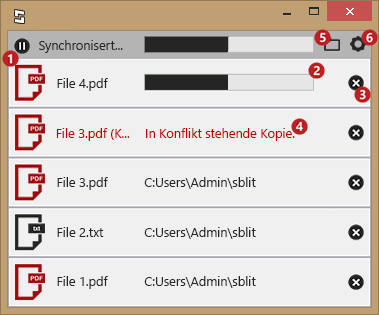
\includegraphics[]{images/systemtray.png}

Mit einem einfachen Klick auf das Icon öffnet sich die Übersicht, in der der
Benutzer auf die folgenden Optionen Zugriff bekommt:

\begin{description}

	\item[{Letzte Änderungen innerhalb des sblit-Ordners}]
		Dem Benutzer wird hier eine Auflistung der zuletzt hinzugefügten Dateien
		geboten. Neben dem an den Dateityp angepassten Bild, wird auch der Dateiname
		und Ordnerpfad angegeben.

	\item[{Fortschrittsbalken laufender Synchronisationsvorgänge}]
		Bei laufenden Synchronisationen hat der User die Möglichkeit, den
		Fortschritt zu verfolgen.

	\item[{Button für das Abbrechen der Synchronisation}]
		Bei irrtümlichem Hinzufügen von Dateien oder Ähnlichem, hat der Benutzer die
		 Möglichkeit, die laufende Synchronisation mithilfe des Löschen-Buttons
		abzubrechen.

	\item[{Anzeige von aufgetretenen Fehlern}]
		Bei Versionskonflikten, die auftreten, wenn 2 Synchronisationspartner die
		selbe Datei gleichzeitig bearbeiten, sowie bei diversen anderen Fehlern,
		wird der User benachrichtigt.

	\item[{Link zum sblit-Ordner}]
		Um dem Benutzer schnellen Zugriff auf seinen konfigurierten sblit-Ordner zu
		gestatten, gibt es den Ordner-Button, mit dem sich der sblit-Ordner im
		Datei-Browser öffnet.

	\item[{Öffnen des Konfigurationsmenüs}]
		Mit einem Klick auf den Optionen-Button öffnet sich das
		\ref{sec:Konfigurationsmenü}.
\end{description}
